% Тут используется класс, установленный на сервере Papeeria. На случай, если
% текст понадобится редактировать где-то в другом месте, рядом лежит файл matmex-diploma-custom.cls
% который в момент своего создания был идентичен классу, установленному на сервере.
% Для того, чтобы им воспользоваться, замените matmex-diploma на matmex-diploma-custom
% Если вы работаете исключительно в Papeeria то мы настоятельно рекомендуем пользоваться
% классом matmex-diploma, поскольку он будет автоматически обновляться по мере внесения корректив
%

% По умолчанию используется шрифт 14 размера. Если нужен 12-й шрифт, уберите опцию [14pt]
%\documentclass[14pt]{matmex-diploma}
\documentclass[14pt]{matmex-diploma-custom}

\usepackage{listings}
\usepackage{minted}
\usepackage{amsmath}
\usepackage{fancyvrb}
\usepackage{color}
\usepackage{pdfpages}
\usepackage{caption}
\usepackage{subcaption}

\renewcommand{\lstlistingname}{Листинг}
\renewcommand\listingscaption{Листинг}

\begin{document}
% Год, город, название университета и факультета предопределены,
% но можно и поменять.

\filltitle{ru}{
    chair              = {Кафедра системного программирования},
    title              = {Динамически формируемый код: синтаксический анализ контекстно-свободной аппроксимации},
    type               = {coursework},
    position           = {студента},
    group              = 444,
    author             = {Ковалев Дмитрий Александрович},
    supervisorPosition = {к.\,ф.-м.\,н., ст.\,преп.},
    supervisor         = {Григорьев С.\,В.},
    reviewerPosition   = {},
    reviewer           = {},
    chairHeadPosition  = {},
    chairHead          = {},
%   university         = {Санкт-Петербургский Государственный Университет},
%   faculty            = {Математико-механический факультет},
%   city               = {Санкт-Петербург},
%   year               = {2013}
}

\maketitle
\tableofcontents
% У введения нет номера главы
\section*{Введение}
Современные языки программирования общего назначения поддерживают возможность работы со строковыми литералами,  позволяя формировать из них выражения при помощи строковых операций. Строковые выражения могут создаваться динамически, с использованием таких конструкций языка, как циклы и условные операторы. Данный подход распространен, например, при формировании SQL-запросов к базам данных из программ, написанных на Java, C$\#$ и других высокоуровневых языках (см. листинг \ref{lst:example}).

\begin{figure}[h!]	
	\lstset{language=[Sharp]C,
		showstringspaces=false,
		basicstyle=\small,
		keywordstyle=\bfseries,,	
	}
	\begin{lstlisting}[caption={Динамически формируемый SQL-запрос}, label={lst:example}, captionpos=b]
private void Example (int cond) {
    string columnName = cond > 42 ? "X" : "Y";
    string queryString = 
        "SELECT name" + columnName + " FROM table";
    Program.ExecuteImmediate(queryString);
}
	\end{lstlisting}
\end{figure}

Недостаток рассматриваемого метода заключается в том, что формируемое выражение, с точки зрения компилятора, является обычной строкой, и, следовательно, не проходит статических проверок на корректность и безопасность, что приводит к ошибкам времени выполнения и усложняет разработку и сопровождение системы. Более того, использование классических методов статического анализа, таких как синтаксический разбор, для динамически формируемых выражений невозможно, так как, в общем случае, они не представимы в виде линейного потока, который принимают на вход традиционные алгоритмы.

Существует несколько подходов, позволяющих частично решать проблему проверки корректности такого вида выражений. Один из них основан на проверке включения языка, генерируемого программой, в язык, заданный пользователем в виде простого перечисления строк, либо при помощи грамматики \cite{jsa, phpsa}. Здесь под языком, который генерирует программа, подразумевается множество значений динамически формируемого выражения, а точнее, некоторая его аппроксимация, ведь в общем случае такое множество может быть рекурсивно перечислимым. Другой подход заключается в проведении синтаксического анализа аппроксимации множества значений \cite{alvor, a_lr}. Стоит отметить, что такой подход позволяет не просто отвечать на вопрос о включении языков, но и реализовать дополнительную функциональность, такую как вычисление семантики, а также, в некоторых случаях, автодополнение и рефакторинг динамически формируемого кода \cite{varis}.

В магистерской диссертации \cite{nastya} был описан алгоритм синтаксического анализа регулярной аппроксимации динамически формируемых выражений на основе алгоритма обобщенного синтаксического анализа GLL \cite{gll} и подробности его реализации в рамках проекта YaccConstructor \cite{yc}. Данное решение обладает несколькими важными достоинствами. Во-первых, результатом работы алгоритма является компактное представление множества деревьев разбора корректных значений выражения (при этом некорректные значения отбрасываются), которое может быть использовано для проведения других видов статического анализа. Во-вторых, реализация представляет собой классический генератор синтаксических анализаторов, что позволяет легко добавлять поддержку новых языков.

Так как большинство языков программирования принадлежит к классу контекстно-свободных, использование регулярной аппроксимации влечет за собой появление синтаксических ошибок, отсутствующих в исходном множестве значений выражения. В данной работе, также выполненной в рамках проекта YaccConstructor, будет представлен алгоритм, который основан на описанной модификации GLL, но позволяет производить синтаксический анализ более точной контекстно-свободной аппроксимации, что ведет к сокращению количества ложных синтаксических ошибок. Также, будет описан процесс получения данной аппроксимации из исходного кода и преобразование ее в форму, пригодную для работы с GLL-анализатором.

\section{Постановка задачи}
Целью дипломной работы является разработка алгоритма синтаксического анализа контекстно-свободной аппроксимации динамически формируемых выражений на базе существующей модификации алгоритма GLL. Для ее достижения были поставлены перечисленные ниже задачи.
\begin{itemize}
    \item Реализовать подходящее для последующего анализа представление контекстно-свободной аппроксимации.
    \item Модифицировать существующий алгоритм синтаксического анализа регулярной аппроксимации, основанный на GLL.   
    \item Провести экспериментальное исследование.
\end{itemize}

\section{Обзор}
В данной секции описываются существующие методы анализа динамически формируемых выражений, в том числе алгоритм синтаксического анализа регулярной аппроксимации, реализованный в проекте YaccConstructor. 
\subsection{Cуществующие инструменты}
Под \textit{регулярной аппроксимацией} далее будем подразумевать регулярное выражение (или соответствующий конечный автомат), аппроксимирующий сверху множество значений динамически формируемого выражения.

В настоящее время существуют два основных подхода к анализу динамически формируемого кода. Первый из них заключается в проверке включения языков. Он позволяет лишь отвечать на вопрос, содержатся ли выражения, генерируемые программой, в эталонном языке, который был задан пользователем при помощи контекстно-свободной грамматики, либо явным перечислением. Следующие инструменты реализуют данный подход. 

\begin{itemize}
    \item \textbf{Java String Analyzer (JSA, \cite{jsa, jsa_url})} --- инструмент для статического анализа строковых выражений в программах, написанных на Java. Для каждого выражения строит регулярную аппроксимацию и проверяет включение языка, генерируемого данной аппроксимацией, в эталонный контекстно-свободный язык.
    \item \textbf{PHP String Analyzer (PHPSA, \cite{phpsa})} --- инструмент для анализа строковых выражений в программах на PHP. Отличается от предыдущего инструмента использованием контекстно-свободной аппроксимации, что позволяет увеличить точность анализа.
\end{itemize}

Второй подход заключается в проведении синтаксического анализа некоторого представления множества значений динамически формируемого выражения.

\begin{itemize}
    \item \textbf{Alvor \cite{alvor}} --- плагин для IDE Eclipse. Позволяет статически проверять корректность SQL-запросов, генерируемых в программах на Java. Для представления множества значений выражения использует понятие абстрактной строки, которая может быть преобразована в конечный автомат над алфавитом токенов исходного языка. Данный автомат затем передается для синтаксического анализа модифицированному GLR-алгоритму. Alvor не поддерживает обработку строковых операций, за исключением конкатенации, и выражений, которые формируются при помощи циклов.
    \item \textbf{Varis \cite{varis}} --- плагин для Eclipse, представлен в 2015 году. Поддерживает анализ выражений на HTML, CSS и JavaScript в программах на PHP. Реализует функции подсветки кода, автодополнения и перехода к объявлению. 
    \item \textbf{Абстрактный синтаксический анализ \cite{a_lr}} --- в данном подходе множество значений выражения описывается при помощи dataflow-уравнений, полученных из исходного кода программы (см. рис. \ref{dataflow_ex}). Эти уравнения затем решаются методом поиска наименьшей неподвижной точки в домене LR-стеков, т.е. одновременно с решением уравнения производится синтаксический анализ с использованием стандартного LR(LALR)-автомата. Результатом анализа является множество LR-стеков, представляющих различные варианты разбора выражения. К сожалению, в статьях, посвященных этому подходу, не было описано эффективное представление результатов, которое могло бы использоваться для более сложных видов анализа.
\end{itemize}

\begin{figure}[h]
    \centering
    \begin{subfigure}{0.45\textwidth}
        \centering
        \begin{minipage}{4cm}
	        \begin{BVerbatim}[commandchars=\\\{\}]
x = \textcolor{red}{"a"}
while ...
    x = \textcolor{red}{"["} . x . \textcolor{red}{"]"}
print x
		    \end{BVerbatim}	
	    \end{minipage}
	\end{subfigure}
	~
	\begin{subfigure}{0.45\textwidth}
	    \centering
	    \begin{minipage}{4cm}
		    \begin{BVerbatim}[commandchars=\\\{\}, codes={\catcode`$=3}]
X0 = \textcolor{red}{a} 
X1 = X0 $\cup$ X2
X2 = \textcolor{red}{[} . X1 . \textcolor{red}{]}
X3 = X1 
		    \end{BVerbatim}
		\end{minipage}
	\end{subfigure}
	\caption{Исходный код и dataflow-уравнения, извлеченные из него}
	\label{dataflow_ex}
\end{figure}

\subsection{YaccConstructor}

YaccConstructor (далее YC, \cite{yc}) --- исследовательский проект лаборатории языковых инструментов  JetBrains на математико-механическом факультете СПбГУ, направленный на исследования в области лексического и синтаксического анализа, а также статического анализа динамически формируемого кода. Проект включает в себя одноименную модульную платформу для разработки лексических и синтаксических анализаторов, содержащую большое количество компонент: язык описания грамматик YARD, преобразования над грамматиками и др. Основным языком разработки является F$\#$.

Ранее, в рамках магистерской диссертации \cite{nastya}, на платформе YC был разработан алгоритм синтаксического анализа регулярной аппроксимации динамически формируемого кода, который позволяет получать компактное представление множества деревьев разбора анализируемого выражения.

\subsection{Алгоритм синтаксического анализа регулярной аппроксимации (YC)}
Предложенный алгоритм является модификацией алгоритма обобщенного синтаксического анализа Generalized LL (GLL, \cite{gll}). Данная модификация принимает на вход не линейный поток токенов, как оригинальный алгоритм, а детерминированный конечный автомат над алфавитом токенов. Данный автомат является результатом работы специальной процедуры лексического анализа над динамически формируемым выражением. Пример такого автомата приведен на рисунке \ref{reg_app_ex}.

Отметим, что построенный автомат может порождать строки, которые не принадлежат множеству значений исходного выражения. В данном примере программа генерирует строки, которые представляют собой правильные скобочные последовательности: \verb+ [a]; [[a]]; ... +. В это же время, множество строк, порождаемых автоматом, содержит, например, такие элементы: \verb+ [a; [[a; [a]] +.

\begin{figure}[t]
    \centering
	\begin{subfigure}{0.4\textwidth}
	    \centering
	    \begin{minipage}{4cm}
		    \begin{Verbatim}[commandchars=\\\{\}]
x = \textcolor{red}{"a"}
while ...
    x = \textcolor{red}{"["} . x . \textcolor{red}{"]"}
print x
		    \end{Verbatim}
		\end{minipage}
	\end{subfigure}
	~
	\begin{subfigure}{0.4\textwidth}
	\centering
		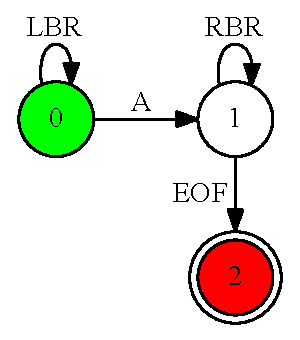
\includegraphics[width=4cm]{pictures/reg_app.pdf}	
	\end{subfigure}
	\caption{Пример регулярной аппроксимации}
	\label{reg_app_ex}
\end{figure}

Результатом работы алгоритма будет сжатое представление леса разбора всех корректных значений выражения --- Shared Packed Parse Forest (SPPF, \cite{sppf}). Под корректными значениями здесь подразумеваются строки, разобранные анализатором, т.е. выводимые во входной грамматике. Так, если провести синтаксический анализ рассматриваемой аппроксимации по грамматике, представленной на рисунке \ref{g_1}, то получится SPPF, изображенный на рисунке \ref{sppf_1}. При этом после завершения работы алгоритма пользователь получит отчет о том, что во время анализа было обнаружено некоторое количество синтаксических ошибок.

Чтобы сократить количество подобных ложных ошибок, необходимо предоставить более точную аппроксимацию исходного множества значений и изменить алгоритм таким образом, чтобы он мог работать с этой аппроксимацией. Этому и будет посвящена данная работа.   

\begin{figure}[t]
\centering
$$
	\begin{array}{crcl}
		&start &::=& s \\
		&s & ::= & \mbox{\texttt{LBR }} s \mbox{\texttt{ RBR }} | \ \mbox{\texttt{A}}\\
	\end{array}
$$
\caption{Грамматика $G_1$}
\label{g_1}
\end{figure}

\begin{figure}[t!]
\centering
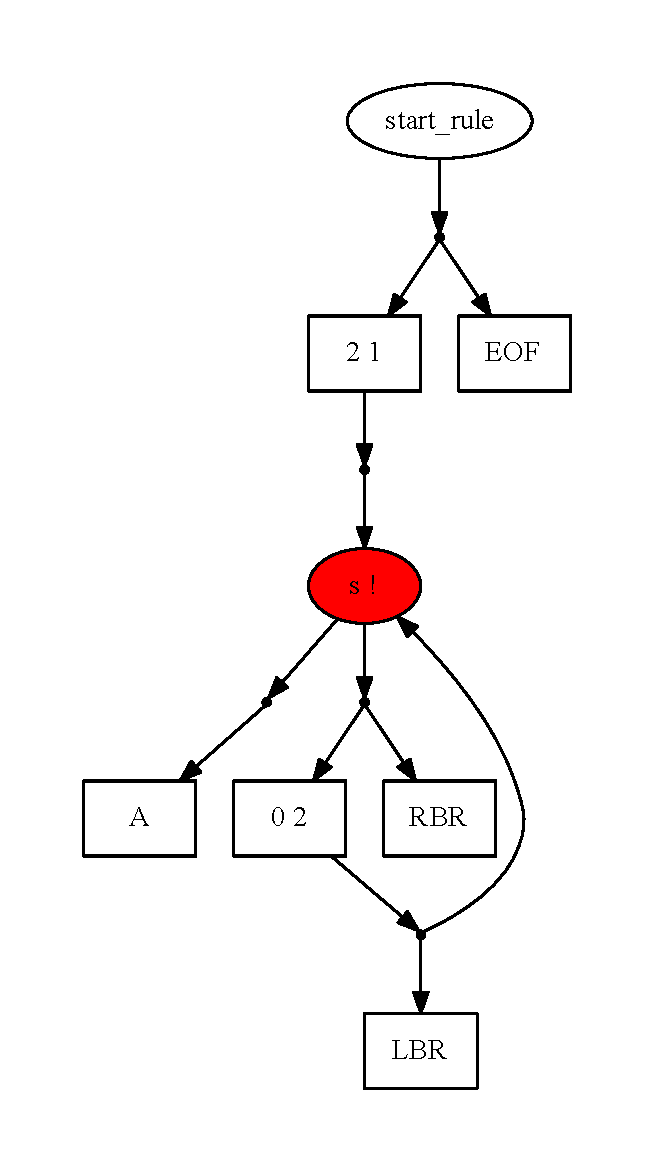
\includegraphics[width=7cm]{pictures/sppf.pdf}
\caption{SPPF для грамматики $G_1$ и автомата с рис. \ref{reg_app_ex}}
\label{sppf_1}
\end{figure}

\section{КС-аппроксимация динамически формируемого выражения}
Вернемся к одному из рассмотренных ранее подходов к анализу динамически формируемого кода. На рисунке \ref{dataflow_ex} был приведен пример dataflow-уравнений, получаемых из исходного кода программы для проведения абстрактного синтаксического анализа. Можно заметить, что данные уравнения представляют собой контекстно-свободную грамматику, где нетерминальные символы --- имена переменных, а терминалы --- строковые литералы (см. рис \ref{eq_gram}). При этом оператор объединения будет означать, что для нетерминала существует несколько продукций.

\begin{figure}[h]
    \centering
	\begin{subfigure}{0.4\textwidth}
	    \centering
	    \begin{minipage}{4cm}
		    \begin{Verbatim}[commandchars=\\\{\}, codes={\catcode`$=3}]
X0 = \textcolor{red}{a} 
X1 = X0 $\cup$ X2
X2 = \textcolor{red}{[} . X1 . \textcolor{red}{]}
X3 = X1 
		    \end{Verbatim}
		\end{minipage}
	\end{subfigure}
	~
	\begin{subfigure}{0.4\textwidth}
	\centering
	    \begin{minipage}{4cm}
		    \begin{Verbatim}[commandchars=\\\{\}]
X0 ::= \textcolor{red}{a}
X1 ::= X0 | X2
X2 ::= \textcolor{red}{[} X1 \textcolor{red}{]} 
X3 ::= X1
		    \end{Verbatim}
		\end{minipage}	
	\end{subfigure}
	\caption{Представление dataflow-уравнений в виде грамматики}
	\label{eq_gram}
\end{figure}

Таким образом, преобразованные dataflow-уравнения можно использовать как контекстно-свободную аппроксимацию динамически формируемого выражения. Для данного примера такая аппроксимация, в отличие от регулярной (рис. \ref{reg_app_ex}), описывает в точности то множество строк, которое генерирует исходная программа.

Предыдущая модификация GLL в проекте YC работает с графовым представлением конечного автомата. Соответственно, для поддержки нового вида аппроксимации необходимо было найти и реализовать удобное для анализа представление КС-грамматики в виде графа.  

\subsection{Grammar Flow Graph}
Такое представление было взято из статьи \cite{gfg}, вышедшей в 2015 году. \textit{Grammar Flow Graph (GFG)} (так авторы, Keshav Pingali и Gianfranco Bilardi, назвали свою разработку) --- это граф с вершинами и ребрами специальных типов, при помощи которого можно смоделировать любую контекстно-свободную грамматику. Пример GFG приведен на рисунке \ref{gfg_ex}. 

\begin{figure}[h]
    \centering
    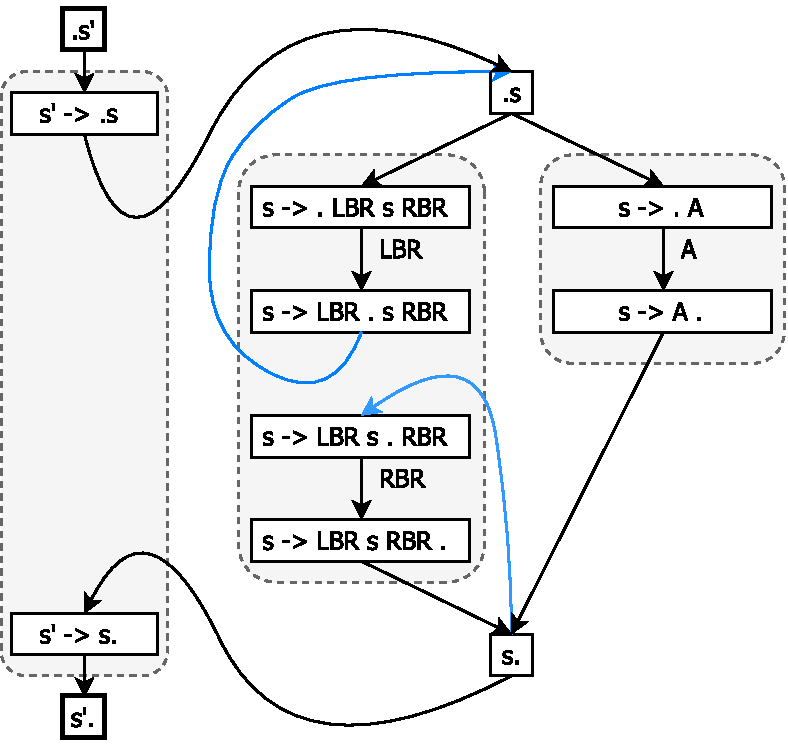
\includegraphics[width=9cm]{pictures/GFG.pdf}
    \caption{GFG для грамматики $G_1$}
    \label{gfg_ex}
\end{figure}


\section{Результаты}

\begin{itemize}
\item Промежуточные результаты.
\begin{itemize}
    \item Написан обзор существующих подходов к анализу динамически формируемых выражений.   
    \item Реализовано внутреннее представление GFG и преобразование грамматик в это представление.
\end{itemize}
\end{itemize}

\begin{itemize}
    \item В ходе дальнейшей работы планируется следующее.
    \begin{itemize}
        \item Модифицировать GLL таким образом, чтобы позволить производить синтаксический анализ GFG.
        \item Провести экспериментальное исследование полученного алгоритма. 
    \end{itemize}
\end{itemize}


\setmonofont[Mapping=tex-text]{CMU Typewriter Text}
\bibliographystyle{ugost2008ls}
\bibliography{diploma.bib}
\end{document}
